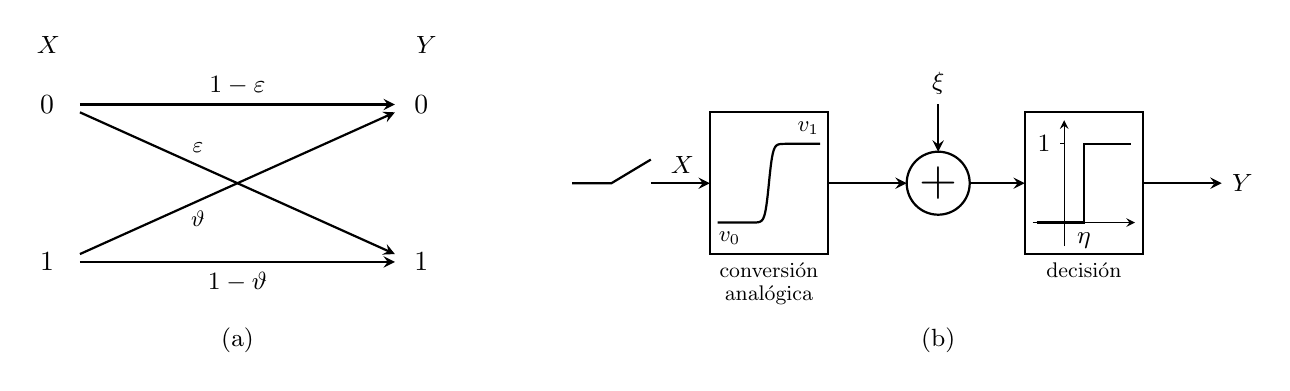
\begin{tikzpicture}
\shorthandoff{>}
%
\begin{scope}
\node at  (-.4,1.75){\small $X$}; \node at  (4.4,1.75){\small $Y$};
%
\draw[>=stealth,->,thick] (-.2,1) node[left]{0} (0,1) -- (4,1) node[right]{\ 0};
\node[above] at (2,1){\small $1-\varepsilon$};
%
\draw[>=stealth,->,thick] (-.2,-1) node[left]{1} (0,-1) -- (4,-1) node[right]{\ 1};
\node[below] at (2,-1){\small $1-\vartheta$};
%
\draw[>=stealth,->,thick] (0,.9)--(4,-.9);
\node[scale=.9] at (1.5,.45){\small $\varepsilon$};
%
\draw[>=stealth,->,thick] (0,-.9)--(4,.9);
\node[scale=.9] at (1.5,-.45){\small $\vartheta$};
%
\end{scope}
%
\begin{scope}[xshift=7cm]
%
% entrada
\draw[thick] (-.75,0)--(-.25,0)--(.25,.3);
\draw[>=stealth,->,thick] (.25,0)--(1,0);
%\draw[>=stealth,->,thick] (.25,-.5) node[below]{\small $X$} --(.25,.1);
\node[above] at (.65,0){\small $X$};
%
% puesta en niveles
\draw[thick] (1,-.9) rectangle (2.5,.9);
\node[scale=.9] at (1.25,-.7){\small $v_0$};
\node[scale=.9] at (2.25,.7){\small $v_1$};
\draw[thick,domain=-4.5:4.5,samples=100] (1.1,-.5) -- plot ({\x/10+1.75},{.5*tanh(2*\x)}) --(2.4,.5);
\node[below,scale=.85] at (1.75,-.9){\small conversi\'on};
\node[below,scale=.85] at (1.75,-1.2){\small anal\'ogica};
%
% adicion del ruido
\draw[>=stealth,->,thick] (2.5,0)--(3.5,0);
\draw[thick] (3.9,0) circle (.4);
\draw[>=stealth,->,thick] (3.9,1) node[above]{\small $\xi$} --(3.9,.4);
\node[align=center,scale=1.5] at (3.9,0){\large +};
%
% decision
\draw[>=stealth,->,thick] (4.3,0)--(5,0);
\draw[thick] (5,-.9) rectangle (6.5,.9);
\draw[>=stealth,->] (5.1,-.5)--(6.4,-.5);
\draw[>=stealth,->] (5.5,-.8)--(5.5,.8);
\draw[thick] (5.15,-.5)--(5.75,-.5)--(5.75,.5)--(6.35,.5);
\node[below] at (5.75,-.5){\small $\eta$};
\draw (5.5,.5)--(5.45,.5) node[left]{\small 1};
\node[below,scale=.85] at (5.75,-.9){\small decisi\'on};
%
% salida
\draw[>=stealth,->,thick] (6.5,0)--(7.5,0) node[right]{\small $Y$};
\end{scope}
\node at (2,-2){\small (a)};
\node at (10.9,-2){\small (b)};
\end{tikzpicture}
